\documentclass[accentcolor=tud0b,12pt,paper=a4]{tudreport}

\usepackage[utf8]{inputenc}
\usepackage{ngerman}
\usepackage{parcolumns}

\newcommand{\titlerow}[2]{
	\begin{parcolumns}[colwidths={1=.15\linewidth}]{2}
		\colchunk[1]{#1:} 
		\colchunk[2]{#2}
	\end{parcolumns}
	\vspace{0.2cm}
}

\title{Open Diabetes UAM Heuristik Algorithm}
\subtitle{Pflichtenheft UAM}
\subsubtitle{%
	\titlerow{Gruppe 11}{%
		Aino Schwarte <aino.schwarte@stud.tu-darmstadt.de>\\
		Anna Mees <anna.mees@stud.tu-darmstadt.de>\\
		Jan Paul Petto <janpaul.petto@stud.tu-darmstadt.de>\\
		Paul Wolfart <paul.wolfart@stud.tu-darmstadt.de>\\
		Tom Großmann <tom.grossmann@stud.tu-darmstadt.de>}
	\titlerow{Teamleiter}{Benedikt Schneider <schneider-benedikt@gmx.net>}
	\titlerow{Auftraggeber}{%
		M.Sc. Jens Heuschkel <heuschkel@tk.tu-darmstadt.de>\\
		Telecooperation\\
		Smart Urban Networks}
	\titlerow{Abgabedatum}{31.03.2019}
\institution{Bachelor-Praktikum WS 2018/2019\\Fachbereich Informatik}}

\begin{document}

	\maketitle
	\tableofcontents 
	\newpage
	\chapter{Zielbestimmung}
	
	Das Projekt Open Diabetes UAM Heuristik Algorithmen entwickelt ein Programm zur richtigen Erkennung von Mahlzeiten anhand von Blutwerten, die in einer Nightscout Datenbank gespeichert sind. 
	%Dies soll das richtige setzen von notwendigen Insulindosen ermöglichen. 
	Nightscout stellt dabei eine Onlineplattform zur grafischen Darstellung der Werte dar. \\

Folgende Punkte müssen implementiert bzw. erstellt werden:\\

\title{\textbf{Must-Have:}}
\begin{itemize}
	\item Skript zum Lesen und Schreiben von Daten in einer Nightscout Instanz	
	\item Kommandozeilentool zum Lesen, Schreiben und Synchronisieren von Nightscout
	\item Parser zum Überführen von Datensätzen aus dem Skript in Java
	\item Algorithmus zur korrekten Berechnung von Kohlenhydraten
	\item Modifikation von Nightscout um angekündigte und berechnete Kohlenhydrate getrennt speichern  zu können.      %und darstellen
	\item Plotten der Daten 
	\item Kommandozeilentool, das Daten einliest und berechnete Kohlenhydrate und Plots ausgibt
	\item Docker-Container der zum Programmstart einen Datensatz einliest, den Algorithmus ausführt und berechnete Kohlenhydrate und Plots ausgibt

	\item Wikiartikel:
	\begin{itemize}
	\item Anleitung für das Kommandozeilentool
	\item Erklärung wie die Daten aus Nightscout auf unsere Daten abgebildet werden
	\item Algorithmen und mögliche Einstellungsfaktoren
	\item Anleitung zum Aufsetzen und Einstellen von lokalen Nightscout Instanze die mit dem Tool funktionieren
	\end{itemize}

\end{itemize}

\title{\textbf{Should-Have:}}

\begin{itemize}	
	\item Nightscout Repository modifizieren 


%* Die Nightscout-Repots sollten modifiziert werden um im Tagesprofil
%** IOB korrekt anzuzeigen
%** COB korrekt anzuzeigen
%** neben dem Zielbereich eine "gelbe" Zone auszuwerten
%** berechnete Carbs anzuzeigen
%* Dokumentation der Nichtscout Modifikationen


	
\end{itemize}
	
	\chapter{Ausgangslage}

Für das Projekt stehen folgende Infrastrukturen zur Verfügung: 
\begin{itemize}
	\item Anonymisierte Patientendaten zum Testen der Ansätze
	\item Nightscout um eigene Instanzen aufzusetzen 
	\item Beschreibungen der Tools
	\item Paper mit Ansätzen zur Berechnung der Insulin- und Kohlenhydratwerte
\end{itemize}
		
	\chapter{Anforderungen}
	\subsection{funktional}
\begin{itemize}
	\item Das Programm muss die Größe der stattfindenden Mahlzeiten (Kohlenhydrate in Gramm) korrekt erkennen. Dabei gilt eine Toleranz von $\pm$6gr, oder 10\%.
	\item  
\end{itemize}
	
	\subsection{nicht-funktional}
\begin{itemize}
	\item Die Datenvisualisierung der Mahlzeiten muss hübsch sein  (lol !!! wird noch geändert !!!!)
\end{itemize}
	
	\chapter{Grobarchitektur}
	
	\centering
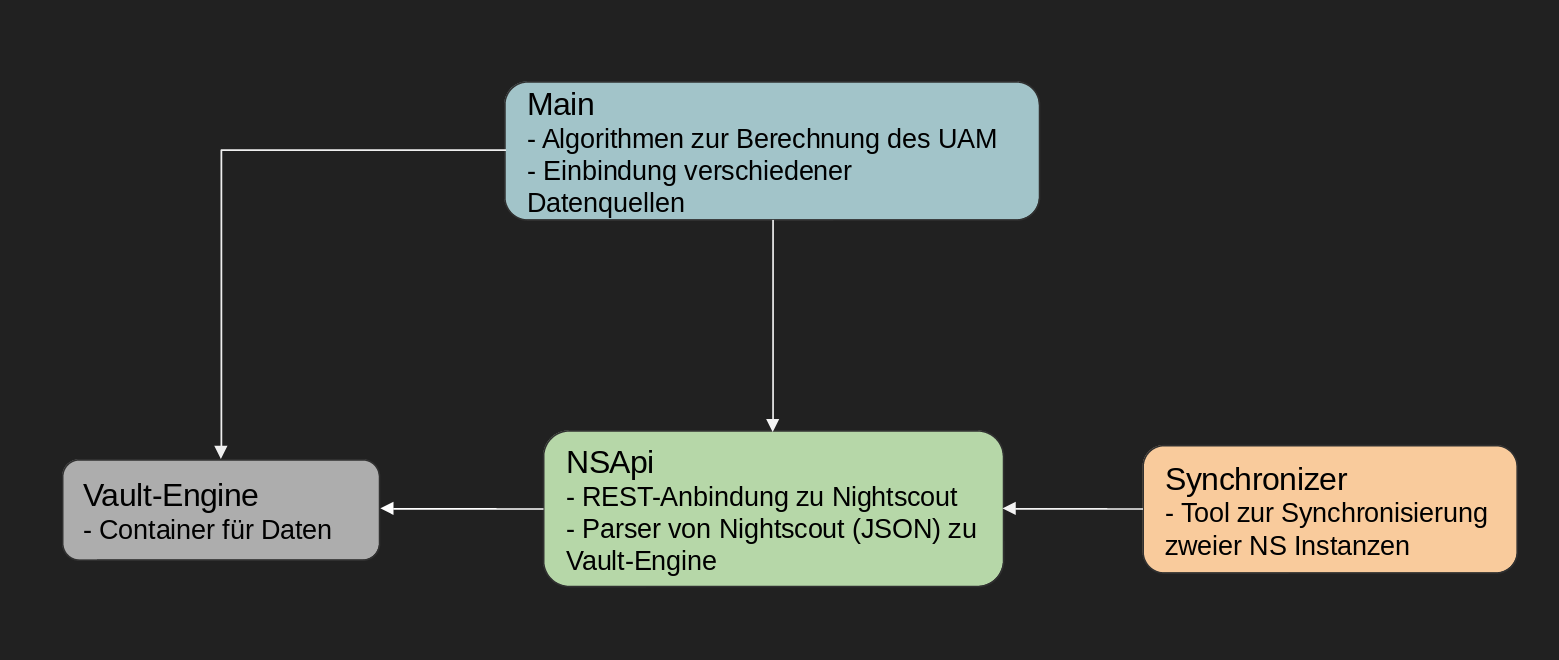
\includegraphics[width=0.7\textwidth]{architektur.png}
	
	\section{Qualitätssicherung}
	Siehe QS-Dokument.
	
	\section{Risikomanagement}
	
	\section{Rechtliches}
	
	Wir entwickeln unter der AGPLv3-Lizenz und verwenden nur Open-Source Quellen. Dadurch vermeiden wir Copy-Right-Verletzungen und schließen jede Garantie an unserem Code aus.
	
\end{document}
